\documentclass[tikz, border=20pt]{standalone}
\usepackage{amsmath}
\usetikzlibrary{arrows.meta, calc, positioning}

\definecolor{pnavy}{HTML}{0E2A47}
\definecolor{pteal}{HTML}{356170}
\definecolor{pgold}{HTML}{B5842A}
\definecolor{pgrey}{HTML}{495057}

\begin{document}
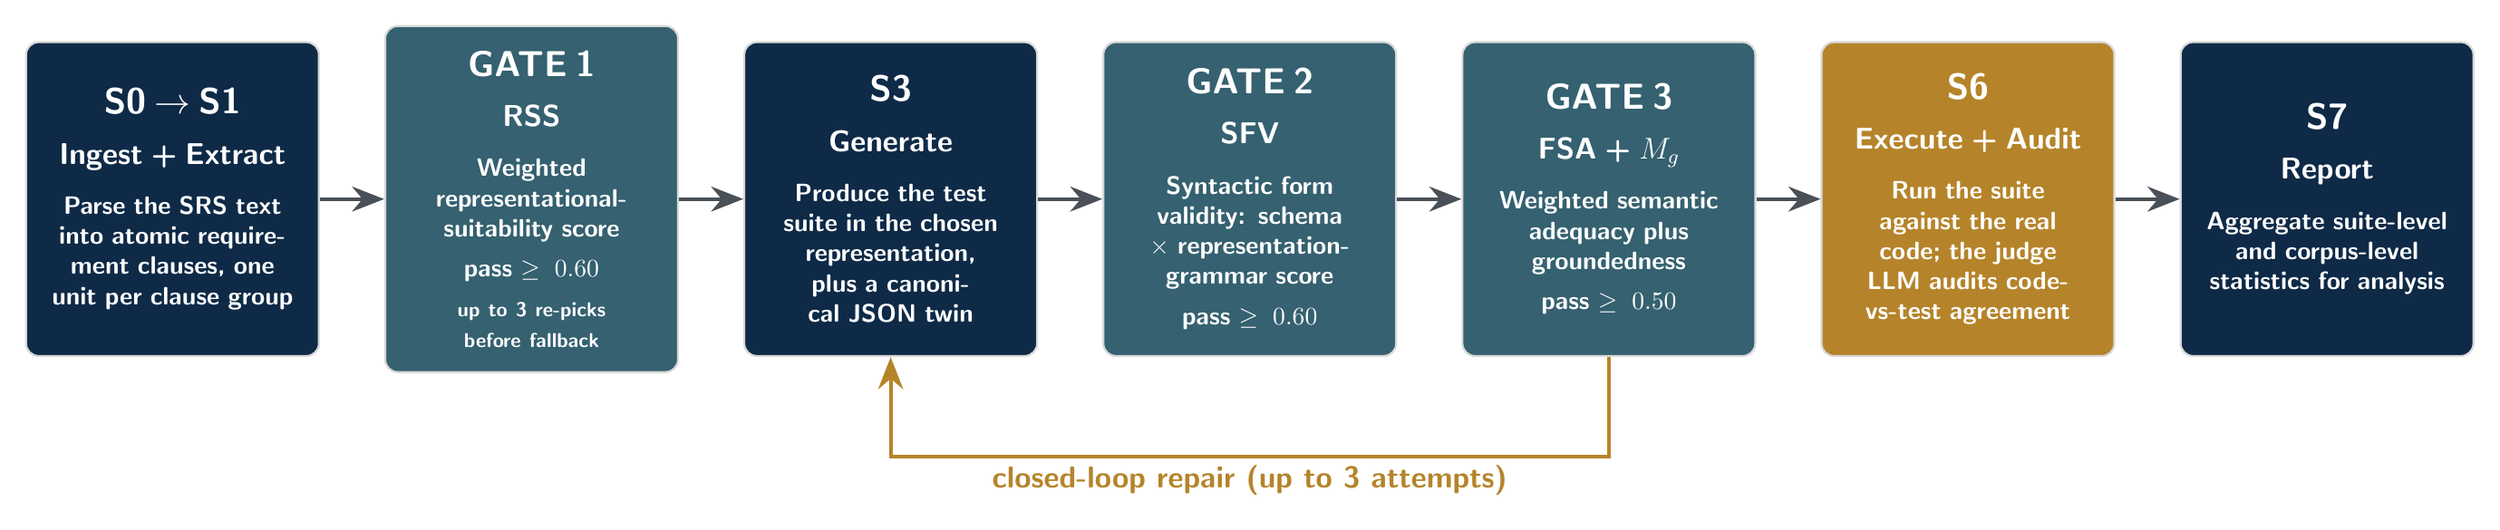
\begin{tikzpicture}[
  font=\sffamily,
  pbox/.style={rectangle, rounded corners=5pt, text=white, align=center,
    text width=3.4cm, minimum height=4.4cm, inner sep=10pt, draw=black!15, thick},
  node distance=9mm,
  arr/.style={-{Stealth[length=4.5mm, width=3.5mm]}, line width=1.4pt, pgrey}
]

\node[pbox, fill=pnavy] (s01)
  {\Large\bfseries S0 $\to$ S1\\[6pt]
   \large\bfseries Ingest + Extract\\[8pt]
   \normalsize Parse the SRS text into atomic requirement clauses, one unit per clause group};

\node[pbox, fill=pteal, right=of s01] (g1)
  {\Large\bfseries GATE 1\\[6pt]
   \large\bfseries RSS\\[8pt]
   \normalsize Weighted representational-suitability score\\[4pt]
   \textbf{pass $\geq 0.60$}\\[4pt]
   \footnotesize up to 3 re-picks before fallback};

\node[pbox, fill=pnavy, right=of g1] (s3)
  {\Large\bfseries S3\\[6pt]
   \large\bfseries Generate\\[8pt]
   \normalsize Produce the test suite in the chosen representation, plus a canonical JSON twin};

\node[pbox, fill=pteal, right=of s3] (g2)
  {\Large\bfseries GATE 2\\[6pt]
   \large\bfseries SFV\\[8pt]
   \normalsize Syntactic form validity: schema $\times$ representation-grammar score\\[4pt]
   \textbf{pass $\geq 0.60$}};

\node[pbox, fill=pteal, right=of g2] (g3)
  {\Large\bfseries GATE 3\\[6pt]
   \large\bfseries FSA + $M_g$\\[8pt]
   \normalsize Weighted semantic adequacy plus groundedness\\[4pt]
   \textbf{pass $\geq 0.50$}};

\node[pbox, fill=pgold, right=of g3] (s6)
  {\Large\bfseries S6\\[6pt]
   \large\bfseries Execute + Audit\\[8pt]
   \normalsize Run the suite against the real code; the judge LLM audits code-vs-test agreement};

\node[pbox, fill=pnavy, right=of s6] (s7)
  {\Large\bfseries S7\\[6pt]
   \large\bfseries Report\\[8pt]
   \normalsize Aggregate suite-level and corpus-level statistics for analysis};

\foreach \a/\b in {s01/g1, g1/s3, s3/g2, g2/g3, g3/s6, s6/s7}
  \draw[arr] (\a.east) -- (\b.west);

\coordinate (dropg3) at ($(g3.south)+(0,-14mm)$);
\coordinate (drops3) at ($(s3.south)+(0,-14mm)$);
\draw[arr, pgold] (g3.south) -- (dropg3) -- (drops3) -- (s3.south);
\node[below, font=\sffamily\bfseries\large, text=pgold] at ($(dropg3)!0.5!(drops3)$) {closed-loop repair (up to 3 attempts)};

\end{tikzpicture}
\end{document}
